\documentclass{article}

\usepackage[margin=0.75in]{geometry}
\usepackage{amsmath,amssymb}
\usepackage{graphicx,float}
\usepackage{multirow,setspace}
\usepackage{natbib,enumerate}
\usepackage{caption}
\usepackage{subcaption}
\usepackage{termcal} 
\usepackage{xcolor}
\usepackage{enumitem}
\usepackage{gensymb}
\usepackage{multicol}
\usepackage{listings}
\usepackage{booktabs}
\usepackage{xurl}
\usepackage{xcolor}
\usepackage{hyperref}


\setlength{\marginparwidth}{2cm}

\renewcommand{\thesection}{\Alph{section}}
\newcommand{\HRule}{\rule{\linewidth}{0.5mm}}
\newcommand{\tab}{\hspace{0.5cm}}
\newcommand{\modref}[1]{(\ref{#1})}

\newcommand{\bbeta}{{\mbox{\boldmath$\beta$}}}
\newcommand{\bmu}{{\mbox{\boldmath$\mu$}}}
\newcommand{\balpha}{{\mbox{\boldmath$\alpha$}}}
\newcommand{\btheta}{{\mbox{\boldmath$\theta$}}}
\newcommand{\bpi}{{\mbox{\boldmath$\pi$}}}
\newcommand{\R}{\texttt{R}}
\newcommand{\Lik}{\mathcal{L}}

\begin{document}

%%% HEADER %%%
	\begin{center}
		\HRule \\[0.1cm]
		\vspace{0.1cm}
		{ \LARGE \bfseries MATH 2625: Biostatistical Methods\\[0.5cm] Homework 4, due Thursday, March 27 } \\[0.1cm]
		\HRule \\[0.1cm]
	\end{center}
	
		Please submit a PDF or .doc version of your homework to Canvas by 3:30pm on the due date. Please type \emph{all} responses. You are encouraged to use \R\ for all calculations.

		Fritze Mayer \& Yu Fan Mei
		
	\section*{Theory}
	\begin{enumerate}
		\item For the Mantel-Haenszel odds ratio estimator applied to matched proportions, $\tilde{\theta} = \frac{n_{21}}{n_{12}}$, an estimate of the uncertainty can be constructed by noting that the variance of the $\log(\tilde{\theta})$ is
		\begin{align*}
			\widehat{Var}\left[\log(\tilde{\theta})\right] = \frac{1}{n_{21}} + \frac{1}{n_{12}}.
		\end{align*}
		Using this, construct an $\alpha$-level confidence interval for $\tilde{\theta}$. State any relevant assumptions.
	\end{enumerate}

	The variance of the $\log(\tilde{\theta})$ transformation is given, but to use the delta method to estimate it, we had to assume that the rows were independent. For an odds ratio with a log-transformation, the confidence interval is given as

	$$\log{\tilde{\theta} } \pm Z_{1 - \alpha/2} * \sqrt{Var(\log(\tilde{\theta})) }.$$

	In order to observe this, we assume that $\log(\tilde{\theta})$ approaches a normal distribution via the central limit theorem. This means we need sufficently large $n$. When we exponentiate to undo the transformation, we get

	$$e^{\log{\tilde{\theta} } \pm Z_{1 - \alpha/2} * \sqrt{Var(\log(\tilde{\theta})) }}.$$

	Then we can substitute $\sqrt{\frac{1}{n_{21}} + \frac{1}{n_{12}}}$ for the standard error of the odds ratio, leaving us with 

	$$e^{\left( \tilde{\theta} \pm Z_{1 - \alpha/2} * \sqrt{\frac{1}{n_{21}} + \frac{1}{n_{12}}} \right)}.$$

	When we write this out fully (using exponent rules to pull out the $\tilde{\theta}$) and substituting it for $\frac{n_{21}}{n_{12}}$, we get

	$$\left( \frac{n_{21}}{n_{12}} e^{\left( -Z_{1 - \alpha / 2} * \sqrt{\frac{1}{n_{21}} + \frac{1}{n_{12}}} \right)}, \frac{n_{21}}{n_{12}} e^{\left(Z_{1 - \alpha / 2} * \sqrt{\frac{1}{n_{21}} + \frac{1}{n_{12}}} \right)} \right) $$

	This is our $\alpha$-level confidence interval for the odds ratio.

	\section*{Case Studies}
	For each of the following case studies, create a structured abstract no longer than 4 pages in length (including figures, tables, and references). The Background section is provided for each and should be included in your write-up. You must write the Methods, Results, and Conclusion sections. Code should be included in an appendix as well.

	\begin{enumerate}
		\item Consider a study that examined maternal stress in utero to subsequent childhood wheezing. The data is in the file \texttt{whz.txt} alongside this assignment. The variable \texttt{wheeze} is coded 1 if the child had repeated wheezing events, 0 if the child did not. The variable \texttt{stress} is coded 1 if the mother had elevated bed time stress and 0 if she did not. The variables \texttt{sex} (1 for female, 0 for male), \texttt{smoker} (1 if the mother smoked during pregnancy, 0 if she did not), and \texttt{atopy} (1 for yes, 0 for no) contain the possible confounders. Adjustments for each possible confounder should be performed separately.
	
	\subsubsection*{Data Structure in \R}
	
	You will need to put the data into $2\times2\times K$ arrays. To do this, we can use the \texttt{table()} command where the first entry is the $X$, the second entry is the $Y$, and the third entry is the $Z$. For example, a properly formatted table with \texttt{sex} as $Z$ can be generated using
	\begin{lstlisting}[language = R]
with(whz, table(stress, wheeze, sex))
	\end{lstlisting}

	
	\item In this case study, you will examine the agreement between primary care physicians and psychiatrists, termed specialty care for this analysis, on a set of five indicators. Each indicator denotes whether primary care or specialty care made contact with agency within a system of care framework for managing pediatric mental health. The data is in the file \texttt{soc.txt} alongside this assignment. The variables \texttt{eduPC}, \texttt{cpsPC}, and \texttt{mhPC} denote whether or not primary care (PC) made contact with the respective agency. The variables \texttt{eduSC}, \texttt{cpsSC}, and \texttt{mhSC} denote whether or not specialty care (SC) made contact with the respective agency.

	\subsubsection*{Data Structure in \R}
	
	The data is structured in the \emph{wide} format where each row corresponds to one subject and columns can correspond to multiple measurements. This structure is useful for making population-averaged tables. Thus to get the population averaged table for one of the agencies, say mental health, we could use the following:
	\begin{lstlisting}[language = R]
with(soc, table(mhPC, mhSC))
	\end{lstlisting}

	\end{enumerate}

	

	\newpage
	\subsection*{Background}
	
	Early childhood wheezing, defined as more than one wheezing event in the first three years of life, can be a precursor to the development of asthma. Early identification of children who may potentially develop asthma could lead to early interventions that mitigate the effects. A study was conducted among an urban Boston cohort of 258 pregnant women. On a single day during the second trimester of pregnancy, each woman collected sputum swabs at five times throughout the day: when she first woke up, two hours after waking up, six hours after waking up, two hours before bed, and right before bed. The level of cortisol, a hormone that can be used to measure stress, was measured from each of these samples. Multiple samples were needed as cortisol level naturally vary through out the day. The mothers were then followed through pregnancy and up through the first three years of the child's life to determine the child wheezed or not. Childhood wheezing can be caused by many factors, such as the sex of the child, whether or not the mother smoked during pregnancy, and genetic factors.
	
	Since cortisol levels should naturally be at their lowest right before bed, we are interested in looking for an association between elevated stress levels right before bed and whether or the child experience repeated wheezing in the first three years of life. However, wheezing in children is sex-linked with typically males experience more wheezing events than females. Also, in utero exposure to nicotine may impact lung development. Finally, genetic factors as measured through the phenotype of maternal atopy (i.e. presence of maternal allergies or asthma) may predispose children to wheezing events.

	\subsection*{Methods}
	258 pregnant women were randomly selected from the Boston area for this cohort study. During their pregnancies, we examined their smoking status as well as their mean cortisol levels during the second trimester. We compared their mean cortisol level throughout the day to their cortisol levels right before going to bed. A significant increase in the mothers’ cortisol levels prior to sleeping compared to throughout the day was indicated as an increase in stress. When the children were three years of age, they were examined to see whether or not they developed a wheeze. We also checked to see whether or not the children showed signs of atopy— a genetic predisposition to developing allergic diseases such as asthma, rhinitis, and eczema, among others.

	To control for the potential interaction of the child’s gender on wheezing results, we stratified results based on whether the child was male or female. We calculated the conditional odds ratios before assessing their homogeneity using a Breslow-Day Test. If appropriate, we then used a Mantel-Haenszel Test to determine whether elevated stress levels before sleeping during pregnancy were associated with the child developing a wheeze. We repeated these analyses for the other confounding variables, stratifying for the smoking status of mothers and atopy in the children. All hypothesis tests were conducted at the nominal level in R.

	\subsection*{Results}
	Among the 258 pregnancies, 127 turned out to be male, while the remaining 131 were female. 212 of the mothers smoked, while 46 did not. 164 of the children were not atopic, while 94 of the children showed some form of atopy. Figure 1 shows the presence and absence of maternal elevated bedtime stress, childhood wheezing, sex, maternal smoking status, and child atopy status for all study participants. 

	\begin{table}[h]
		\centering
		\captionsetup{labelformat=empty}
		\footnotesize
		\caption{Tables 1 \& 2: Two-Way Tables Comparing Maternal Stress \& Wheezing in Children}
		\begin{minipage}{0.48\linewidth}
			\centering
			\textbf{Male Children} \\[2pt]
			\begin{tabular}{cccc} % Changed to cccc (no vertical bars)
				\toprule
				\textbf{Maternal Stress} & \textbf{No Wheezing} & \textbf{Wheezing} & \textbf{Total} \\
				\midrule
				Yes & 100 & 8 & 108 \\
				No & 13 & 6 & 19 \\
				\midrule
				\textbf{Total} & 113 & 14 & 127 \\
				\bottomrule
			\end{tabular}
		\end{minipage}
		\hfill
		\begin{minipage}{0.48\linewidth}
			\centering
			\textbf{Female Children} \\[2pt]
			\begin{tabular}{cccc} % Changed to cccc (no vertical bars)
				\toprule
				\textbf{Maternal Stress} & \textbf{No Wheezing} & \textbf{Wheezing} & \textbf{Total} \\
				\midrule
				Yes & 107 & 7 & 114 \\
				No & 16 & 1 & 17 \\
				\midrule
				\textbf{Total} & 123 & 8 & 131 \\
				\bottomrule
			\end{tabular}
		\end{minipage}
	\end{table}
	
	
	
	\newpage
	\begin{figure}[h!]
		\centering
		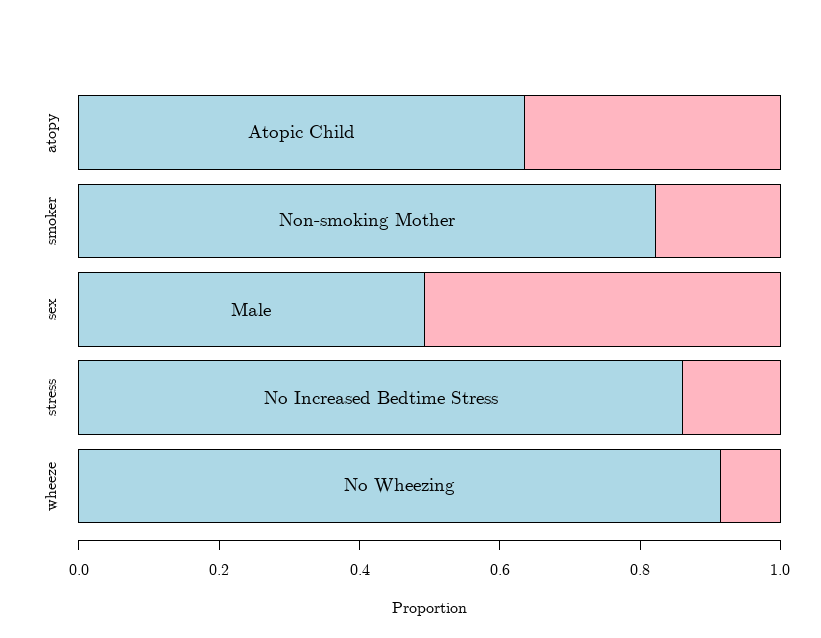
\includegraphics[width=0.6\textwidth]{graphs/stackedBars_case1.png}
		\caption{Proportions of Variables of Interest in Children in the Study \& Their Mothers}
		\label{fig:histogram}
	\end{figure}

	In our study, we found that among male children, the odds of wheezing given mothers showed elevated bedtime stress were 5.77 times greater than if their mothers did not. For female children, the odds of a child wheezing if their mother had elevated bedtime stress were 0.96 times as likely as the odds if their mothers did not have elevated bedtime stress. We found that these odds between sexes were homogenous $(p = 0.134, \chi^2 = 2.243, df = 1)$. After adjustment for sex, we found that the odds of wheezing were significantly higher among children whose mothers had increased bedtime stress during pregnancy than those whose mothers did not show increased bedtime stress during pregnancy ($p = 0.0134$, OR = 3.31, 95\% CI = (1.240, 8.834), CMH $\chi^2 = 6.100)$.


	The odds of wheezing in children whose mothers did not smoke during pregnancy and experienced elevated bedtime stress were 2.78 times greater than in children whose mothers did not experience stress and did not smoke. For children with mothers smoked during pregnancy, the odds of wheezing with mothers who experienced elevated bedtime stress were 10.39 times more than for mothers who did not experience bedtime stress. The Breslow-Day Test confirmed that these odds were homogenous $(p = 0.3395, \chi^2 = 0.9122, df = 1)$. When we adjusted for the confounding influence of maternal smoking, we found that the odds of wheezing were significantly higher among children whose mothers had increased bedtime stress during pregnancy than those whose mothers did not show increased bedtime stress during pregnancy ($p=0.0097$, OR = 3.38, 95\% CI = (1.298, 9.374), CMH $\chi^2 = 6.693)$.

	\begin{table}[h]
		\centering
		\captionsetup{labelformat=empty}
		\footnotesize
		\caption{Tables 3 \& 4: Two-Way Tables Comparing Maternal Stress \& Childhood Wheezing, Adjusted for Smoking Status}
		\begin{minipage}{0.48\linewidth}
			\centering
			\textbf{Mother Smoked During Pregnancy} \\[2pt]
			\begin{tabular}{cccc} % No vertical bars
				\toprule
				\textbf{Stress Level} & \textbf{No Wheezing} & \textbf{Wheezing} & \textbf{Total} \\
				\midrule
				No Stress & 171 & 14 & 185 \\
				Stress & 22 & 5 & 27 \\
				\midrule
				\textbf{Total} & 193 & 19 & 212 \\
				\bottomrule
			\end{tabular}
		\end{minipage}
		\hfill
		\begin{minipage}{0.48\linewidth}
			\centering
			\textbf{Mother did not Smoke During Pregnancy} \\[2pt]
			\begin{tabular}{cccc} % No vertical bars
				\toprule
				\textbf{Stress Level} & \textbf{No Wheezing} & \textbf{Wheezing} & \textbf{Total} \\
				\midrule
				No Stress & 36 & 1 & 37 \\
				Stress & 7 & 2 & 9 \\
				\midrule
				\textbf{Total} & 43 & 3 & 46 \\
				\bottomrule
			\end{tabular}
		\end{minipage}
	\end{table}

	For children without atopy, the odds of wheezing given mothers who experienced elevated bedtime stress were 3.750 times higher than for those with mothers who did not experience stress. In children with atopy, the odds of wheezing given mothers who experienced elevated bed time stress were  2.769 times greater than for those children with mothers who did not experience stress. We found that these odds between smoking statuses of mothers were homogenous $(p = 0.7638, \chi^2 = 0.0903, df = 1)$.  After adjustment for childrens atopy status, we found that the common odds of wheezing were significantly higher among children whose mothers had increased bedtime stress during pregnancy than those whose mothers did not show increased bedtime stress during pregnancy ($p=0.0131$, OR = 3.27, 95\% CI = (1.229, 8.721), CMH $\chi^2 = 6.1498$).

	\begin{table}[h]
		\centering
		\captionsetup{labelformat=empty}
		\footnotesize
		\caption{Tables 5 \& 6: Two-Way Tables Comparing Maternal Stress \& Childhood Wheezing, Stratified by Atopy Status}
		\begin{minipage}{0.48\linewidth}
			\centering
			\textbf{Children without Atopy} \\[2pt]
			\begin{tabular}{cccc} % No vertical bars
				\toprule
				\textbf{Stress Level} & \textbf{No Wheezing} & \textbf{Wheezing} & \textbf{Total} \\
				\midrule
				No Stress & 135 & 9 & 144 \\
				Stress & 16 & 4 & 20 \\
				\midrule
				\textbf{Total} & 151 & 13 & 164 \\
				\bottomrule
			\end{tabular}
		\end{minipage}
		\hfill
		\begin{minipage}{0.48\linewidth}
			\centering
			\textbf{Children with Atopy} \\[2pt]
			\begin{tabular}{cccc} % No vertical bars
				\toprule
				\textbf{Stress Level} & \textbf{No Wheezing} & \textbf{Wheezing} & \textbf{Total} \\
				\midrule
				No Stress & 72 & 6 & 78 \\
				Stress & 13 & 3 & 16 \\
				\midrule
				\textbf{Total} & 85 & 9 & 94 \\
				\bottomrule
			\end{tabular}
		\end{minipage}
	\end{table}

	\subsection*{Discussion}
	We observed a significant association between elevated bedtime stress of mothers during pregnancy and their children developing wheezing. This association held after adjusting for the interaction of various confounders— sex of the child, smoking status of the mothers during pregnancy, and even atopy in the children. These findings suggest that maternal stress is associated with childhood respiratory health as measured by childhood wheezing. These results are consistent with other findings, which suggest that maternal stress is associated with the development of wheezing and asthma (Van de Loo et. al., 2015).
	
	One limitation of this study was the locality, with all participants being from the Boston area. Follow-up research should seek to confirm these results with other regions. Additionally, it may be worth exploring other potential negative health outcomes related to maternal stress. Other studies have suggested that maternal stress has a negative impact on the resulting learning ability \& motor development of children, among many other unidentified outcomes (DiPietro, 2004). Clinical research should also seek to find ways to mitigate maternal stress.

	\newpage
	\subsection*{Appendix}

	\begin{itemize}
		\item DiPietro, J. A. (2004). The role of prenatal maternal stress in child development. \textit{Current Directions in Psychological Science}, \textit{13}(2), 71-74.
		\item van de Loo, K. F., van Gelder, M. M., Roukema, J., Roeleveld, N., Merkus, P. J., \& Verhaak, C. M. (2015). Prenatal maternal psychological stress and childhood asthma and wheezing: a meta-analysis. \textit{European Respiratory Journal}, \textit{47}(1), 133-146.
	\end{itemize}

	\subsection*{R Code}
	\begin{lstlisting}[
		language=R, 
		label={lst:condOR_analysis}, 
		xleftmargin=\parindent,   % Align with paragraph indentation
		linewidth=\textwidth,     % Ensure it fits within text width
		frame=tb,                 % Optional: frame only top and bottom
		breaklines=true           % Wrap long lines instead of cutting off
	]
	## 1 ##
	library(DescTools)
	library(epitools)
	source('ORFun.R')
	
	whz <- read.table('whz.txt', header=TRUE, sep='')
	
	tab_sex <- with(whz, table(stress, wheeze, sex))
	tab_smoke <- with(whz, table(stress, wheeze, smoker))
	tab_atopy <- with(whz, table(stress, wheeze, atopy))
	
	condOR(tab_sex)     
	condOR(tab_smoke)   
	condOR(tab_atopy)
	
	BreslowDayTest(tab_sex)
	BreslowDayTest(tab_smoke)
	BreslowDayTest(tab_atopy)
	
	mantelhaen.test(tab_sex, correct = FALSE)
	mantelhaen.test(tab_smoke, correct = FALSE)
	mantelhaen.test(tab_atopy, correct = FALSE)
	
	## bar charts for case study 1
	prop_ones <- colMeans(whz)  # 1s
	prop_zeros <- 1 - prop_ones  # 0s
	
	prop_matrix <- rbind(prop_zeros, prop_ones)
	
	bar_positions <- barplot(prop_matrix, col = c('lightblue', 'lightpink'), 
							 names.arg = names(whz), 
							 main = '', 
							 xlab = 'Proportion', 
							 horiz = TRUE,  # horizontal chart
							 xlim = c(0, 1))
	
	custom_labels <- c('No Wheezing', 
					   'No Increased Bedtime Stress', 
					   'Male', 
					   'Non-smoking Mother',
					   'Atopic Child') 
	# labels are so people know what the blue and red mean
	
	text(y = bar_positions, x = prop_zeros / 2,
		 labels = custom_labels, col = 'black', cex = 1.2, font = 2)
	\end{lstlisting}





	\newpage
	\subsection*{Background}
	Many children are treated for mental health disorders in primary care settings.  The system of care (SOC) provides a framework for collaboration among pediatric mental health providers, but it is unclear if youth treated for mental health disorders in primary care receive such coordination.  At the South Boston Community Health Center from 9/2012-8/2013 for 74 individuals $<$18 years, the odds of contact with SOC agencies (the mental health system, the education system, child protective services, the juvenile justice system and developmental disability services) were compared for mental health treatment in primary versus specialty care.  The odds of SOC contact within primary care compared to specialty care specifically for contact with mental health, education and child protective services were examined.  As care coordination may improve health outcomes, increased support and education for care coordination specific to youth treated for mental health disorders in primary care settings may be warranted.
	
	Due to sparsity in two of outcomes (contact with the juvenile justice system and contact with developmental disability services), our study focuses on three agencies: the mental health system (MH), the education system (EDU), and child protective services (CPS). Specifically, we want to examine possible differences between contact with each of the agencies for primary care compared to specialty care. Each subject was seen first by a primary care physician and, later, by a specialty care physician. Specialty care was not made aware of the agencies primary care had recommended contact with. 

	\subsection*{Methods}
	In this study, we examined the diagnoses of 74 minors who visited the South Boston Community Health Center from July 2012 to August 2013. The subjects visited both a primary care physician as well as a specialty care physician. To avoid information bias \& misclassification, primary and specialty physicians were not made aware of the decisions made by the other. We were primarily interested in whether or not the physicians chose to contact the three relevant institutions: the Massachusetts Department of Mental Health (MH), the child’s school or school district, and CPS. Due to the small number of cases available, we compared the matched odds of contact with each of the three agencies among primary care and specialty care physicians and then examined whether or not the difference was significant using a binomial exact test. All testing was done in R at the nominal level.

	\subsection*{Results}
	In regards to mental health services, primary care physicians contacted the Department of Mental Health in 16 of the cases, while specialty care physicians contacted the MH in 24 of the 74 cases. We found discordance in 16 total cases, 4 where PC contacted the MH and SC did not, and 12 where PC did not contact the MH and SC did. While the odds of a PC physician contacting MH was 66.7\% lower the odds of a SC physician contacting MH (Matched OR = 0.333,  95\% CI = [0.108, 1.034]), we did not find this difference to be statistically significant ($p = 0.0768$, $\hat{p} = 0.25$, 95\% CI = (0.073, 0.524)).



	\begin{table}[h]
		\centering
		\footnotesize
		\captionsetup{labelformat=empty}
		\caption{Table 1. Comparison of Cases Where Primary \& Specialty Care Contacted Department of Mental Health}
		\renewcommand{\arraystretch}{1.2}
		\begin{tabular}{llccc}
			\toprule
			& & \multicolumn{2}{c}{\textbf{SC Contacts MH}} & \\  
			\cmidrule(lr){3-4}
			& & \textbf{No} & \textbf{Yes} & \textbf{Total} \\  
			\midrule
			\multirow{2}{*}{\textbf{PC Contacts MH}} & \textbf{No} & 46 & 12 & 58 \\  
			& \textbf{Yes} & 4 & 12 & 16 \\  
			\midrule
			& \textbf{Total} & 50 & 24 & 74 \\  
			\bottomrule
		\end{tabular}
		\label{tab:pc_sc_mh}
	\end{table}


	Primary care physicians contacted school systems in only 13 of the 74 cases, while for specialty care physicians, this number was 42 cases. As shown in Table 2, we observed 31 cases where SC officials contacted school systems when PC did not, and only 2 cases where the opposite occurred— PC contacted schools and SC did not. We found that primary physicians were 93.5\% less likely than specialty physicians to contact education systems (Matched OR = 0.065, 95\% CI = [0.015, 0.270]). This result was statistically significant ($p < 0.0001, \hat{p} = 0.0606$, 95\% CI = (0.0074, 0.2023)), suggesting that primary physicians were less likely to reach out to schools than specialty physicians.

	\newpage
	\begin{table}[h]
		\centering
		\footnotesize
		\captionsetup{labelformat=empty}
		\caption{Table 2. Comparison of Cases Where Primary \& Specialty Care Contacted School System}
		\renewcommand{\arraystretch}{1.2}
		\begin{tabular}{llccc}
			\toprule
			& & \multicolumn{2}{c}{\textbf{SC Contacts EDU}} & \\  
			\cmidrule(lr){3-4}
			& & \textbf{No} & \textbf{Yes} & \textbf{Total} \\  
			\midrule
			\multirow{2}{*}{\textbf{PC Contacts EDU}} & \textbf{No} & 30 & 31 & 61 \\  
			& \textbf{Yes} & 2 & 11 & 13 \\  
			\midrule
			& \textbf{Total} & 32 & 42 & 74 \\  
			\bottomrule
		\end{tabular}
		\label{tab:pc_sc_edu}
	\end{table}

	Primary care physicians contacted child protective services in 7 of the 74 cases, while specialty care physicians contacted CPS in 10 cases. In 7 cases, SC contacted CPS where PC did not, while in 4 cases, SC did not contact CPS and PC did. The odds of a primary care physician contacting CPS were 42.9\% lower than the odds of a specialty care physician doing the same (Matched OR = 0.571,  95\% CI = [0.167, 1.952]). However, we found that this observed difference was not statistically significant ($p = 0.5488, \hat{p} = 0.3636$, 95\% CI = (0.1092, 0.6920)).

	\begin{table}[h]
		\centering
		\footnotesize
		\captionsetup{labelformat=empty}
		\caption{Table 3. Comparison of Cases Where Primary \& Specialty Care Contacted Child Protective Services}
		\renewcommand{\arraystretch}{1.2}
		\begin{tabular}{llccc}
			\toprule
			& & \multicolumn{2}{c}{\textbf{SC Contacts CPS}} & \\  
			\cmidrule(lr){3-4}
			& & \textbf{No} & \textbf{Yes} & \textbf{Total} \\  
			\midrule
			\multirow{2}{*}{\textbf{PC Contacts CPS}} & \textbf{No} & 60 & 7 & 67 \\  
			& \textbf{Yes} & 4 & 3 & 7 \\  
			\midrule
			& \textbf{Total} & 64 & 10 & 74 \\  
			\bottomrule
		\end{tabular}
		\label{tab:pc_sc_cps}
	\end{table}

	\subsection*{Discussion}
	We only observed a significant difference in contact rates between primary care and specialty care physicians when it came to contacting schools. Specifically, primary care physicians were far less likely to contact a child’s school system than secondary care physicians. This indicates a gap in care coordination between primary and specialty care physicians. This is consistent with findings from similar studies (Porras-Javier et al., 2018), as specialty care physicians may have additional training related to developmental pediatrics and behavioral health. They may also have more experience in working directly with school systems, in contrast to primary care physicians, who receive a more general medical training (Donohoe, 1998). Since many children are treated through primary care, changes to training should be made to allow primary care physicians to better serve the needs of children.

	Further studies should be conducted to understand such differences across related departments and systems, including social service programs \& agencies in other states. One of the limitations of this study was its containment within one clinic in the Boston area. We also faced issues with finding cases, as not many children see both a primary care and secondary care physician. Future research should look into examining a larger number of cases. Additionally, it may be worth looking into potential confounders in the physicians’ decision-making process. Some noteworthy issues to consider include implicit bias related to race, gender or socioeconomic status, parental influence, or even the age of the children being examined, among many other factors.

	\newpage
	\subsection*{Appendix}
	\begin{itemize}
		\item Donohoe, M. T. (1998). Comparing generalist and specialty care: discrepancies, deficiencies, and excesses. \textit{Archives of Internal Medicine}, 158(15), 1596--1608.
		
		\item Porras-Javier, L., Bromley, E., Lopez, M., et al. (2018). Challenges to Effective Primary Care-Specialty Communication and Coordination in the Mental Health Referral and Care Process for Publicly Insured Children. \textit{J Behav Health Serv Res}, 45, 668--677. \url{https://doi.org/10.1007/s11414-018-9585-z}
	\end{itemize}

	\subsection*{R Code}
	\begin{lstlisting}[
		language=R, 
		label={lst:matchedOR_analysis}, 
		xleftmargin=\parindent,   % Align with paragraph indentation
		linewidth=\textwidth,     % Ensure it fits within text width
		frame=tb,                 % Optional: frame only top and bottom
		breaklines=true           % Wrap long lines instead of cutting off
	]
	## 2 ##
	library(DescTools)
	library(epitools)
	source('ORFun.R')
	
	soc <- read.table('soc.txt', header=TRUE)
	
	### mh ###
	tab_mh <- with(soc, table(mhPC, mhSC))
	n21     <- 4
	n12     <- 12
	theta   <- n21/n12
	
	oddsratio.matched(n21, n12)
	binom.test(n21, n21 + n12, p = 0.5)
	
	
	### edu ###
	tab_edu <- with(soc, table(eduPC, eduSC))
	
	n21     <- 2
	n12     <- 31
	theta   <- n21/n12
	
	oddsratio.matched(n21, n12)
	binom.test(n21, n21 + n12, p = 0.5)
	
	
	### cps ###
	
	tab_cps <- with(soc, table(cpsPC, cspSC))
	
	n21     <- 4
	n12     <- 7
	theta   <- n21/n12
	
	oddsratio.matched(n21, n12)
	binom.test(n21, n21 + n12, p = 0.5)
	
	
	
	### matched odds ratio method
	### run this before case study 2
	### couldn't find an OR method in epi tools for matched
	### so resorted to this
	oddsratio.matched <- function(n21, n12, conf_level = 0.95) {
	  or_value <- n21 / n12
	  
	  # standard error for CI
	  se_log_or <- sqrt(1/n21 + 1/n12)
	  
	  # z score for CI
	  z_score <- qnorm(1 - (1 - conf_level) / 2)
	  
	  log_or <- log(or_value)
	  lower_log_or <- log_or - z_score * se_log_or
	  upper_log_or <- log_or + z_score * se_log_or
	  
	  # untransform ci
	  lower_or <- exp(lower_log_or)
	  upper_or <- exp(upper_log_or)
	  
	  # code for printing
	  or_value <- round(or_value, 7)
	  lower_or <- round(lower_or, 7)
	  upper_or <- round(upper_or, 7)
	  
	  output_text <- paste(
		'Matched-pairs odds ratio (', 
		conf_level * 100, '% confidence interval)\n', 
		'OR: ', or_value, '\n', 
		'Lower    Upper\n', 
		lower_or, '    ', upper_or,
		sep = ''
	  )
	  
	  # print
	  cat(output_text)
	}
	\end{lstlisting}
	




	
		
\end{document}














